\documentclass[1p]{elsarticle_modified}
%\bibliographystyle{elsarticle-num}

%\usepackage[colorlinks]{hyperref}
%\usepackage{abbrmath_seonhwa} %\Abb, \Ascr, \Acal ,\Abf, \Afrak
\usepackage{amsfonts}
\usepackage{amssymb}
\usepackage{amsmath}
\usepackage{amsthm}
\usepackage{scalefnt}
\usepackage{amsbsy}
\usepackage{kotex}
\usepackage{caption}
\usepackage{subfig}
\usepackage{color}
\usepackage{graphicx}
\usepackage{xcolor} %% white, black, red, green, blue, cyan, magenta, yellow
\usepackage{float}
\usepackage{setspace}
\usepackage{hyperref}

\usepackage{tikz}
\usetikzlibrary{arrows}

\usepackage{multirow}
\usepackage{array} % fixed length table
\usepackage{hhline}

%%%%%%%%%%%%%%%%%%%%%
\makeatletter
\renewcommand*\env@matrix[1][\arraystretch]{%
	\edef\arraystretch{#1}%
	\hskip -\arraycolsep
	\let\@ifnextchar\new@ifnextchar
	\array{*\c@MaxMatrixCols c}}
\makeatother %https://tex.stackexchange.com/questions/14071/how-can-i-increase-the-line-spacing-in-a-matrix
%%%%%%%%%%%%%%%

\usepackage[normalem]{ulem}

\newcommand{\msout}[1]{\ifmmode\text{\sout{\ensuremath{#1}}}\else\sout{#1}\fi}
%SOURCE: \msout is \stkout macro in https://tex.stackexchange.com/questions/20609/strikeout-in-math-mode

\newcommand{\cancel}[1]{
	\ifmmode
	{\color{red}\msout{#1}}
	\else
	{\color{red}\sout{#1}}
	\fi
}

\newcommand{\add}[1]{
	{\color{blue}\uwave{#1}}
}

\newcommand{\replace}[2]{
	\ifmmode
	{\color{red}\msout{#1}}{\color{blue}\uwave{#2}}
	\else
	{\color{red}\sout{#1}}{\color{blue}\uwave{#2}}
	\fi
}

\newcommand{\Sol}{\mathcal{S}} %segment
\newcommand{\D}{D} %diagram
\newcommand{\A}{\mathcal{A}} %arc


%%%%%%%%%%%%%%%%%%%%%%%%%%%%%5 test

\def\sl{\operatorname{\textup{SL}}(2,\Cbb)}
\def\psl{\operatorname{\textup{PSL}}(2,\Cbb)}
\def\quan{\mkern 1mu \triangleright \mkern 1mu}

\theoremstyle{definition}
\newtheorem{thm}{Theorem}[section]
\newtheorem{prop}[thm]{Proposition}
\newtheorem{lem}[thm]{Lemma}
\newtheorem{ques}[thm]{Question}
\newtheorem{cor}[thm]{Corollary}
\newtheorem{defn}[thm]{Definition}
\newtheorem{exam}[thm]{Example}
\newtheorem{rmk}[thm]{Remark}
\newtheorem{alg}[thm]{Algorithm}

\newcommand{\I}{\sqrt{-1}}
\begin{document}

%\begin{frontmatter}
%
%\title{Boundary parabolic representations of knots up to 8 crossings}
%
%%% Group authors per affiliation:
%\author{Yunhi Cho} 
%\address{Department of Mathematics, University of Seoul, Seoul, Korea}
%\ead{yhcho@uos.ac.kr}
%
%
%\author{Seonhwa Kim} %\fnref{s_kim}}
%\address{Center for Geometry and Physics, Institute for Basic Science, Pohang, 37673, Korea}
%\ead{ryeona17@ibs.re.kr}
%
%\author{Hyuk Kim}
%\address{Department of Mathematical Sciences, Seoul National University, Seoul 08826, Korea}
%\ead{hyukkim@snu.ac.kr}
%
%\author{Seokbeom Yoon}
%\address{Department of Mathematical Sciences, Seoul National University, Seoul, 08826,  Korea}
%\ead{sbyoon15@snu.ac.kr}
%
%\begin{abstract}
%We find all boundary parabolic representation of knots up to 8 crossings.
%
%\end{abstract}
%\begin{keyword}
%    \MSC[2010] 57M25 
%\end{keyword}
%
%\end{frontmatter}

%\linenumbers
%\tableofcontents
%
\newcommand\colored[1]{\textcolor{white}{\rule[-0.35ex]{0.8em}{1.4ex}}\kern-0.8em\color{red} #1}%
%\newcommand\colored[1]{\textcolor{white}{ #1}\kern-2.17ex	\textcolor{white}{ #1}\kern-1.81ex	\textcolor{white}{ #1}\kern-2.15ex\color{red}#1	}

{\Large $\underline{12a_{0568}~(K12a_{0568})}$}

\setlength{\tabcolsep}{10pt}
\renewcommand{\arraystretch}{1.6}
\vspace{1cm}\begin{tabular}{m{100pt}>{\centering\arraybackslash}m{274pt}}
\multirow{5}{120pt}{
	\centering
	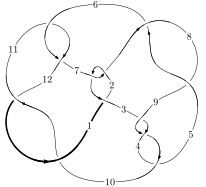
\includegraphics[width=112pt]{../../../GIT/diagram.site/Diagrams/png/1369_12a_0568.png}\\
\ \ \ A knot diagram\footnotemark}&
\allowdisplaybreaks
\textbf{Linearized knot diagam} \\
\cline{2-2}
 &
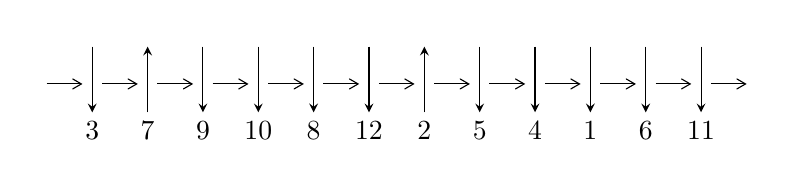
\begin{tikzpicture}[x=20pt, y=17pt]
	% nodes
	\node (C0) at (0, 0) {};
	\node (C1) at (1, 0) {};
	\node (C1U) at (1, +1) {};
	\node (C1D) at (1, -1) {3};

	\node (C2) at (2, 0) {};
	\node (C2U) at (2, +1) {};
	\node (C2D) at (2, -1) {7};

	\node (C3) at (3, 0) {};
	\node (C3U) at (3, +1) {};
	\node (C3D) at (3, -1) {9};

	\node (C4) at (4, 0) {};
	\node (C4U) at (4, +1) {};
	\node (C4D) at (4, -1) {10};

	\node (C5) at (5, 0) {};
	\node (C5U) at (5, +1) {};
	\node (C5D) at (5, -1) {8};

	\node (C6) at (6, 0) {};
	\node (C6U) at (6, +1) {};
	\node (C6D) at (6, -1) {12};

	\node (C7) at (7, 0) {};
	\node (C7U) at (7, +1) {};
	\node (C7D) at (7, -1) {2};

	\node (C8) at (8, 0) {};
	\node (C8U) at (8, +1) {};
	\node (C8D) at (8, -1) {5};

	\node (C9) at (9, 0) {};
	\node (C9U) at (9, +1) {};
	\node (C9D) at (9, -1) {4};

	\node (C10) at (10, 0) {};
	\node (C10U) at (10, +1) {};
	\node (C10D) at (10, -1) {1};

	\node (C11) at (11, 0) {};
	\node (C11U) at (11, +1) {};
	\node (C11D) at (11, -1) {6};

	\node (C12) at (12, 0) {};
	\node (C12U) at (12, +1) {};
	\node (C12D) at (12, -1) {11};
	\node (C13) at (13, 0) {};

	% arrows
	\draw[->,>={angle 60}]
	(C0) edge (C1) (C1) edge (C2) (C2) edge (C3) (C3) edge (C4) (C4) edge (C5) (C5) edge (C6) (C6) edge (C7) (C7) edge (C8) (C8) edge (C9) (C9) edge (C10) (C10) edge (C11) (C11) edge (C12) (C12) edge (C13) ;	\draw[->,>=stealth]
	(C1U) edge (C1D) (C2D) edge (C2U) (C3U) edge (C3D) (C4U) edge (C4D) (C5U) edge (C5D) (C6U) edge (C6D) (C7D) edge (C7U) (C8U) edge (C8D) (C9U) edge (C9D) (C10U) edge (C10D) (C11U) edge (C11D) (C12U) edge (C12D) ;
	\end{tikzpicture} \\
\hhline{~~} \\& 
\textbf{Solving Sequence} \\ \cline{2-2} 
 &
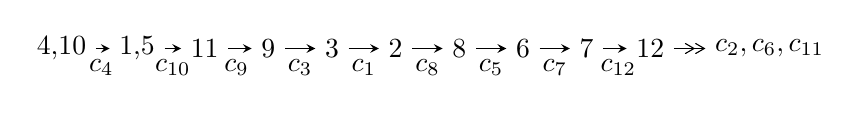
\begin{tikzpicture}[x=23pt, y=7pt]
	% node
	\node (A0) at (-1/8, 0) {4,10};
	\node (A1) at (17/16, 0) {1,5};
	\node (A2) at (17/8, 0) {11};
	\node (A3) at (25/8, 0) {9};
	\node (A4) at (33/8, 0) {3};
	\node (A5) at (41/8, 0) {2};
	\node (A6) at (49/8, 0) {8};
	\node (A7) at (57/8, 0) {6};
	\node (A8) at (65/8, 0) {7};
	\node (A9) at (73/8, 0) {12};
	\node (C1) at (1/2, -1) {$c_{4}$};
	\node (C2) at (13/8, -1) {$c_{10}$};
	\node (C3) at (21/8, -1) {$c_{9}$};
	\node (C4) at (29/8, -1) {$c_{3}$};
	\node (C5) at (37/8, -1) {$c_{1}$};
	\node (C6) at (45/8, -1) {$c_{8}$};
	\node (C7) at (53/8, -1) {$c_{5}$};
	\node (C8) at (61/8, -1) {$c_{7}$};
	\node (C9) at (69/8, -1) {$c_{12}$};
	\node (A10) at (11, 0) {$c_{2},c_{6},c_{11}$};

	% edge
	\draw[->,>=stealth]	
	(A0) edge (A1) (A1) edge (A2) (A2) edge (A3) (A3) edge (A4) (A4) edge (A5) (A5) edge (A6) (A6) edge (A7) (A7) edge (A8) (A8) edge (A9) ;
	\draw[->>,>={angle 60}]	
	(A9) edge (A10);
\end{tikzpicture} \\ 

\end{tabular} \\

\footnotetext{
The image of knot diagram is generated by the software ``\textbf{Draw programme}" developed by Andrew Bartholomew(\url{http://www.layer8.co.uk/maths/draw/index.htm\#Running-draw}), where we modified some parts for our purpose(\url{https://github.com/CATsTAILs/LinksPainter}).
}\phantom \\ \newline 
\centering \textbf{Ideals for irreducible components\footnotemark of $X_{\text{par}}$} 
 
\begin{align*}
I^u_{1}&=\langle 
6.14215\times10^{45} u^{89}-3.30510\times10^{45} u^{88}+\cdots+8.82311\times10^{45} b-2.12797\times10^{46},\\
\phantom{I^u_{1}}&\phantom{= \langle  }-3.98658\times10^{46} u^{89}+5.02790\times10^{46} u^{88}+\cdots+8.82311\times10^{45} a+2.64205\times10^{47},\;u^{90}- u^{89}+\cdots-11 u-1\rangle \\
I^u_{2}&=\langle 
u^4 a+u^4-2 u^2 a-2 u^2+b- a,\;- u^5 a+3 u^3 a- u^4+a^2-2 a u+3 u^2-2,\;u^6-3 u^4+2 u^2+1\rangle \\
\\
\end{align*}
\raggedright * 2 irreducible components of $\dim_{\mathbb{C}}=0$, with total 102 representations.\\
\footnotetext{All coefficients of polynomials are rational numbers. But the coefficients are sometimes approximated in decimal forms when there is not enough margin.}
\newpage
\renewcommand{\arraystretch}{1}
\centering \section*{I. $I^u_{1}= \langle 6.14\times10^{45} u^{89}-3.31\times10^{45} u^{88}+\cdots+8.82\times10^{45} b-2.13\times10^{46},\;-3.99\times10^{46} u^{89}+5.03\times10^{46} u^{88}+\cdots+8.82\times10^{45} a+2.64\times10^{47},\;u^{90}- u^{89}+\cdots-11 u-1 \rangle$}
\flushleft \textbf{(i) Arc colorings}\\
\begin{tabular}{m{7pt} m{180pt} m{7pt} m{180pt} }
\flushright $a_{4}=$&$\begin{pmatrix}1\\0\end{pmatrix}$ \\
\flushright $a_{10}=$&$\begin{pmatrix}0\\u\end{pmatrix}$ \\
\flushright $a_{1}=$&$\begin{pmatrix}4.51834 u^{89}-5.69856 u^{88}+\cdots-157.416 u-29.9447\\-0.696143 u^{89}+0.374596 u^{88}+\cdots+4.22395 u+2.41181\end{pmatrix}$ \\
\flushright $a_{5}=$&$\begin{pmatrix}1\\u^2\end{pmatrix}$ \\
\flushright $a_{11}=$&$\begin{pmatrix}5.71831 u^{89}-7.17155 u^{88}+\cdots-186.704 u-44.7259\\-1.66422 u^{89}-0.736261 u^{88}+\cdots-37.5768 u-5.22880\end{pmatrix}$ \\
\flushright $a_{9}=$&$\begin{pmatrix}u\\u\end{pmatrix}$ \\
\flushright $a_{3}=$&$\begin{pmatrix}- u^2+1\\- u^2\end{pmatrix}$ \\
\flushright $a_{2}=$&$\begin{pmatrix}4.57115 u^{89}-6.31172 u^{88}+\cdots-163.112 u-31.9782\\-1.06131 u^{89}-0.301013 u^{88}+\cdots-1.47856 u+1.93140\end{pmatrix}$ \\
\flushright $a_{8}=$&$\begin{pmatrix}- u^3+2 u\\- u^5+u^3+u\end{pmatrix}$ \\
\flushright $a_{6}=$&$\begin{pmatrix}u^6-3 u^4+2 u^2+1\\u^8-2 u^6+2 u^2\end{pmatrix}$ \\
\flushright $a_{7}=$&$\begin{pmatrix}3.67198 u^{89}-3.85942 u^{88}+\cdots-90.2360 u-27.2951\\2.09638 u^{89}-0.675864 u^{88}+\cdots-16.6943 u-4.75859\end{pmatrix}$ \\
\flushright $a_{12}=$&$\begin{pmatrix}5.32448 u^{89}-6.50749 u^{88}+\cdots-171.372 u-42.3482\\-1.29912 u^{89}-0.713830 u^{88}+\cdots-34.4333 u-4.88931\end{pmatrix}$\\&\end{tabular}
\flushleft \textbf{(ii) Obstruction class $= -1$}\\~\\
\flushleft \textbf{(iii) Cusp Shapes $= 4.10870 u^{89}-2.12548 u^{88}+\cdots-53.7193 u-31.3376$}\\~\\
\newpage\renewcommand{\arraystretch}{1}
\flushleft \textbf{(iv) u-Polynomials at the component}\newline \\
\begin{tabular}{m{50pt}|m{274pt}}
Crossings & \hspace{64pt}u-Polynomials at each crossing \\
\hline $$\begin{aligned}c_{1}\end{aligned}$$&$\begin{aligned}
&u^{90}+41 u^{89}+\cdots-69 u+1
\end{aligned}$\\
\hline $$\begin{aligned}c_{2},c_{7}\end{aligned}$$&$\begin{aligned}
&u^{90}+u^{89}+\cdots+13 u-1
\end{aligned}$\\
\hline $$\begin{aligned}c_{3},c_{4},c_{9}\end{aligned}$$&$\begin{aligned}
&u^{90}+u^{89}+\cdots+11 u-1
\end{aligned}$\\
\hline $$\begin{aligned}c_{5},c_{8}\end{aligned}$$&$\begin{aligned}
&u^{90}-3 u^{89}+\cdots-10133 u+783
\end{aligned}$\\
\hline $$\begin{aligned}c_{6},c_{11}\end{aligned}$$&$\begin{aligned}
&u^{90}+u^{89}+\cdots+9 u-5
\end{aligned}$\\
\hline $$\begin{aligned}c_{10},c_{12}\end{aligned}$$&$\begin{aligned}
&u^{90}+29 u^{89}+\cdots+471 u+25
\end{aligned}$\\
\hline
\end{tabular}\\~\\
\newpage\renewcommand{\arraystretch}{1}
\flushleft \textbf{(v) Riley Polynomials at the component}\newline \\
\begin{tabular}{m{50pt}|m{274pt}}
Crossings & \hspace{64pt}Riley Polynomials at each crossing \\
\hline $$\begin{aligned}c_{1}\end{aligned}$$&$\begin{aligned}
&y^{90}+29 y^{89}+\cdots-1117 y+1
\end{aligned}$\\
\hline $$\begin{aligned}c_{2},c_{7}\end{aligned}$$&$\begin{aligned}
&y^{90}+41 y^{89}+\cdots-69 y+1
\end{aligned}$\\
\hline $$\begin{aligned}c_{3},c_{4},c_{9}\end{aligned}$$&$\begin{aligned}
&y^{90}-75 y^{89}+\cdots-89 y+1
\end{aligned}$\\
\hline $$\begin{aligned}c_{5},c_{8}\end{aligned}$$&$\begin{aligned}
&y^{90}+65 y^{89}+\cdots-60583609 y+613089
\end{aligned}$\\
\hline $$\begin{aligned}c_{6},c_{11}\end{aligned}$$&$\begin{aligned}
&y^{90}-29 y^{89}+\cdots-471 y+25
\end{aligned}$\\
\hline $$\begin{aligned}c_{10},c_{12}\end{aligned}$$&$\begin{aligned}
&y^{90}+71 y^{89}+\cdots-78091 y+625
\end{aligned}$\\
\hline
\end{tabular}\\~\\
\newpage\flushleft \textbf{(vi) Complex Volumes and Cusp Shapes}
$$\begin{array}{c|c|c}  
\text{Solutions to }I^u_{1}& \I (\text{vol} + \sqrt{-1}CS) & \text{Cusp shape}\\
 \hline 
\begin{aligned}
u &= -0.063363 + 0.857170 I \\
a &= -1.60157 - 0.02571 I \\
b &= -0.981273 + 0.593879 I\end{aligned}
 & \phantom{-}9.60013 - 0.30151 I & -1.10817 + 1.54965 I \\ \hline\begin{aligned}
u &= -0.063363 - 0.857170 I \\
a &= -1.60157 + 0.02571 I \\
b &= -0.981273 - 0.593879 I\end{aligned}
 & \phantom{-}9.60013 + 0.30151 I & -1.10817 - 1.54965 I \\ \hline\begin{aligned}
u &= \phantom{-}0.118441 + 0.851139 I \\
a &= \phantom{-}1.49393 - 0.11981 I \\
b &= \phantom{-}0.898638 + 0.842251 I\end{aligned}
 & \phantom{-}7.97578 - 5.92214 I & -2.87748 + 3.29056 I \\ \hline\begin{aligned}
u &= \phantom{-}0.118441 - 0.851139 I \\
a &= \phantom{-}1.49393 + 0.11981 I \\
b &= \phantom{-}0.898638 - 0.842251 I\end{aligned}
 & \phantom{-}7.97578 + 5.92214 I & -2.87748 - 3.29056 I \\ \hline\begin{aligned}
u &= -0.138419 + 0.847253 I \\
a &= \phantom{-}1.90893 + 0.26202 I \\
b &= \phantom{-}1.129030 - 0.755146 I\end{aligned}
 & \phantom{-}6.97122 + 12.03910 I & -4.54855 - 8.02805 I \\ \hline\begin{aligned}
u &= -0.138419 - 0.847253 I \\
a &= \phantom{-}1.90893 - 0.26202 I \\
b &= \phantom{-}1.129030 + 0.755146 I\end{aligned}
 & \phantom{-}6.97122 - 12.03910 I & -4.54855 + 8.02805 I \\ \hline\begin{aligned}
u &= \phantom{-}0.089333 + 0.853199 I \\
a &= -1.84826 + 0.20136 I \\
b &= -1.141640 - 0.418693 I\end{aligned}
 & \phantom{-}9.00366 - 5.86140 I & -1.98243 + 3.66515 I \\ \hline\begin{aligned}
u &= \phantom{-}0.089333 - 0.853199 I \\
a &= -1.84826 - 0.20136 I \\
b &= -1.141640 + 0.418693 I\end{aligned}
 & \phantom{-}9.00366 + 5.86140 I & -1.98243 - 3.66515 I \\ \hline\begin{aligned}
u &= -1.109560 + 0.413438 I \\
a &= -0.120973 + 1.369430 I \\
b &= \phantom{-}0.098202 + 0.474134 I\end{aligned}
 & \phantom{-}3.99789 - 7.50254 I & \phantom{-0.000000 } 0 \\ \hline\begin{aligned}
u &= -1.109560 - 0.413438 I \\
a &= -0.120973 - 1.369430 I \\
b &= \phantom{-}0.098202 - 0.474134 I\end{aligned}
 & \phantom{-}3.99789 + 7.50254 I & \phantom{-0.000000 } 0\\
 \hline 
 \end{array}$$\newpage$$\begin{array}{c|c|c}  
\text{Solutions to }I^u_{1}& \I (\text{vol} + \sqrt{-1}CS) & \text{Cusp shape}\\
 \hline 
\begin{aligned}
u &= \phantom{-}1.182370 + 0.122207 I \\
a &= \phantom{-}0.100406 + 0.432195 I \\
b &= \phantom{-}1.193500 + 0.510369 I\end{aligned}
 & -1.82140 - 0.65010 I & \phantom{-0.000000 } 0 \\ \hline\begin{aligned}
u &= \phantom{-}1.182370 - 0.122207 I \\
a &= \phantom{-}0.100406 - 0.432195 I \\
b &= \phantom{-}1.193500 - 0.510369 I\end{aligned}
 & -1.82140 + 0.65010 I & \phantom{-0.000000 } 0 \\ \hline\begin{aligned}
u &= \phantom{-}0.041756 + 0.807032 I \\
a &= -0.159012 - 0.738937 I \\
b &= \phantom{-}0.036451 + 0.424290 I\end{aligned}
 & \phantom{-}4.52384 - 2.64817 I & -1.47152 + 3.33157 I \\ \hline\begin{aligned}
u &= \phantom{-}0.041756 - 0.807032 I \\
a &= -0.159012 + 0.738937 I \\
b &= \phantom{-}0.036451 - 0.424290 I\end{aligned}
 & \phantom{-}4.52384 + 2.64817 I & -1.47152 - 3.33157 I \\ \hline\begin{aligned}
u &= -0.097470 + 0.785464 I \\
a &= \phantom{-}0.82289 + 1.43240 I \\
b &= \phantom{-}0.563552 - 0.155489 I\end{aligned}
 & \phantom{-}0.42228 + 5.90745 I & -7.85230 - 6.60506 I \\ \hline\begin{aligned}
u &= -0.097470 - 0.785464 I \\
a &= \phantom{-}0.82289 - 1.43240 I \\
b &= \phantom{-}0.563552 + 0.155489 I\end{aligned}
 & \phantom{-}0.42228 - 5.90745 I & -7.85230 + 6.60506 I \\ \hline\begin{aligned}
u &= \phantom{-}1.138980 + 0.412263 I \\
a &= -0.194847 - 1.067110 I \\
b &= \phantom{-}0.271357 - 0.244873 I\end{aligned}
 & \phantom{-}4.84987 + 1.38168 I & \phantom{-0.000000 } 0 \\ \hline\begin{aligned}
u &= \phantom{-}1.138980 - 0.412263 I \\
a &= -0.194847 + 1.067110 I \\
b &= \phantom{-}0.271357 + 0.244873 I\end{aligned}
 & \phantom{-}4.84987 - 1.38168 I & \phantom{-0.000000 } 0 \\ \hline\begin{aligned}
u &= -1.174040 + 0.310051 I \\
a &= \phantom{-}0.760441 + 0.711639 I \\
b &= \phantom{-}1.23530 + 0.88131 I\end{aligned}
 & -2.83425 - 1.91319 I & \phantom{-0.000000 } 0 \\ \hline\begin{aligned}
u &= -1.174040 - 0.310051 I \\
a &= \phantom{-}0.760441 - 0.711639 I \\
b &= \phantom{-}1.23530 - 0.88131 I\end{aligned}
 & -2.83425 + 1.91319 I & \phantom{-0.000000 } 0\\
 \hline 
 \end{array}$$\newpage$$\begin{array}{c|c|c}  
\text{Solutions to }I^u_{1}& \I (\text{vol} + \sqrt{-1}CS) & \text{Cusp shape}\\
 \hline 
\begin{aligned}
u &= -0.021656 + 0.777387 I \\
a &= \phantom{-}1.64509 + 0.25611 I \\
b &= \phantom{-}1.77954 + 0.17094 I\end{aligned}
 & \phantom{-}2.06022 + 2.77574 I & -4.04299 - 3.19683 I \\ \hline\begin{aligned}
u &= -0.021656 - 0.777387 I \\
a &= \phantom{-}1.64509 - 0.25611 I \\
b &= \phantom{-}1.77954 - 0.17094 I\end{aligned}
 & \phantom{-}2.06022 - 2.77574 I & -4.04299 + 3.19683 I \\ \hline\begin{aligned}
u &= -0.582202 + 0.482242 I \\
a &= \phantom{-}1.56154 - 1.15042 I \\
b &= \phantom{-}0.641273 - 0.707070 I\end{aligned}
 & \phantom{-}2.15933 + 7.36357 I & -6.87028 - 8.54868 I \\ \hline\begin{aligned}
u &= -0.582202 - 0.482242 I \\
a &= \phantom{-}1.56154 + 1.15042 I \\
b &= \phantom{-}0.641273 + 0.707070 I\end{aligned}
 & \phantom{-}2.15933 - 7.36357 I & -6.87028 + 8.54868 I \\ \hline\begin{aligned}
u &= \phantom{-}1.176580 + 0.408870 I \\
a &= \phantom{-}0.202086 + 1.238210 I \\
b &= \phantom{-}0.535480 + 0.478102 I\end{aligned}
 & \phantom{-}5.66669 + 1.33161 I & \phantom{-0.000000 } 0 \\ \hline\begin{aligned}
u &= \phantom{-}1.176580 - 0.408870 I \\
a &= \phantom{-}0.202086 - 1.238210 I \\
b &= \phantom{-}0.535480 - 0.478102 I\end{aligned}
 & \phantom{-}5.66669 - 1.33161 I & \phantom{-0.000000 } 0 \\ \hline\begin{aligned}
u &= -0.005141 + 0.749243 I \\
a &= -1.11720 + 1.29527 I \\
b &= -0.296478 + 0.005780 I\end{aligned}
 & \phantom{-}1.47758 - 1.34536 I & -4.73272 + 0.56742 I \\ \hline\begin{aligned}
u &= -0.005141 - 0.749243 I \\
a &= -1.11720 - 1.29527 I \\
b &= -0.296478 - 0.005780 I\end{aligned}
 & \phantom{-}1.47758 + 1.34536 I & -4.73272 - 0.56742 I \\ \hline\begin{aligned}
u &= -1.260060 + 0.057506 I \\
a &= -0.008082 - 0.481249 I \\
b &= -1.90367 - 0.70076 I\end{aligned}
 & -4.87070 + 2.52144 I & \phantom{-0.000000 } 0 \\ \hline\begin{aligned}
u &= -1.260060 - 0.057506 I \\
a &= -0.008082 + 0.481249 I \\
b &= -1.90367 + 0.70076 I\end{aligned}
 & -4.87070 - 2.52144 I & \phantom{-0.000000 } 0\\
 \hline 
 \end{array}$$\newpage$$\begin{array}{c|c|c}  
\text{Solutions to }I^u_{1}& \I (\text{vol} + \sqrt{-1}CS) & \text{Cusp shape}\\
 \hline 
\begin{aligned}
u &= -1.205890 + 0.409098 I \\
a &= \phantom{-}0.314677 - 1.064430 I \\
b &= \phantom{-}0.378068 - 0.298950 I\end{aligned}
 & \phantom{-}6.08340 + 4.84091 I & \phantom{-0.000000 } 0 \\ \hline\begin{aligned}
u &= -1.205890 - 0.409098 I \\
a &= \phantom{-}0.314677 + 1.064430 I \\
b &= \phantom{-}0.378068 + 0.298950 I\end{aligned}
 & \phantom{-}6.08340 - 4.84091 I & \phantom{-0.000000 } 0 \\ \hline\begin{aligned}
u &= \phantom{-}0.520473 + 0.500551 I \\
a &= \phantom{-}1.17156 + 1.23439 I \\
b &= \phantom{-}0.524177 + 0.800626 I\end{aligned}
 & \phantom{-}2.66978 - 1.59618 I & -5.41754 + 3.51950 I \\ \hline\begin{aligned}
u &= \phantom{-}0.520473 - 0.500551 I \\
a &= \phantom{-}1.17156 - 1.23439 I \\
b &= \phantom{-}0.524177 - 0.800626 I\end{aligned}
 & \phantom{-}2.66978 + 1.59618 I & -5.41754 - 3.51950 I \\ \hline\begin{aligned}
u &= \phantom{-}1.230560 + 0.352038 I \\
a &= \phantom{-}0.445034 - 0.089140 I \\
b &= \phantom{-}1.54264 - 0.03383 I\end{aligned}
 & \phantom{-}0.86290 - 1.52902 I & \phantom{-0.000000 } 0 \\ \hline\begin{aligned}
u &= \phantom{-}1.230560 - 0.352038 I \\
a &= \phantom{-}0.445034 + 0.089140 I \\
b &= \phantom{-}1.54264 + 0.03383 I\end{aligned}
 & \phantom{-}0.86290 + 1.52902 I & \phantom{-0.000000 } 0 \\ \hline\begin{aligned}
u &= -0.386151 + 0.600663 I \\
a &= -1.37669 + 1.32407 I \\
b &= -0.260073 + 0.690515 I\end{aligned}
 & \phantom{-}2.78195 - 3.49276 I & -4.88676 + 2.39495 I \\ \hline\begin{aligned}
u &= -0.386151 - 0.600663 I \\
a &= -1.37669 - 1.32407 I \\
b &= -0.260073 - 0.690515 I\end{aligned}
 & \phantom{-}2.78195 + 3.49276 I & -4.88676 - 2.39495 I \\ \hline\begin{aligned}
u &= -1.285160 + 0.169868 I \\
a &= \phantom{-}0.1170600 - 0.0114062 I \\
b &= -1.096790 - 0.353976 I\end{aligned}
 & -4.98736 + 2.80353 I & \phantom{-0.000000 } 0 \\ \hline\begin{aligned}
u &= -1.285160 - 0.169868 I \\
a &= \phantom{-}0.1170600 + 0.0114062 I \\
b &= -1.096790 + 0.353976 I\end{aligned}
 & -4.98736 - 2.80353 I & \phantom{-0.000000 } 0\\
 \hline 
 \end{array}$$\newpage$$\begin{array}{c|c|c}  
\text{Solutions to }I^u_{1}& \I (\text{vol} + \sqrt{-1}CS) & \text{Cusp shape}\\
 \hline 
\begin{aligned}
u &= \phantom{-}1.297550 + 0.009629 I \\
a &= -0.505550 - 0.905163 I \\
b &= -3.00177 - 1.14994 I\end{aligned}
 & -6.16458 - 2.17147 I & \phantom{-0.000000 } 0 \\ \hline\begin{aligned}
u &= \phantom{-}1.297550 - 0.009629 I \\
a &= -0.505550 + 0.905163 I \\
b &= -3.00177 + 1.14994 I\end{aligned}
 & -6.16458 + 2.17147 I & \phantom{-0.000000 } 0 \\ \hline\begin{aligned}
u &= -1.255600 + 0.330283 I \\
a &= -0.133760 + 0.939798 I \\
b &= -1.95449 - 0.44736 I\end{aligned}
 & -1.75554 + 1.21643 I & \phantom{-0.000000 } 0 \\ \hline\begin{aligned}
u &= -1.255600 - 0.330283 I \\
a &= -0.133760 - 0.939798 I \\
b &= -1.95449 + 0.44736 I\end{aligned}
 & -1.75554 - 1.21643 I & \phantom{-0.000000 } 0 \\ \hline\begin{aligned}
u &= -1.286820 + 0.199890 I \\
a &= \phantom{-}0.543186 - 0.643193 I \\
b &= \phantom{-}1.58806 - 0.78450 I\end{aligned}
 & -2.98447 + 4.84215 I & \phantom{-0.000000 } 0 \\ \hline\begin{aligned}
u &= -1.286820 - 0.199890 I \\
a &= \phantom{-}0.543186 + 0.643193 I \\
b &= \phantom{-}1.58806 + 0.78450 I\end{aligned}
 & -2.98447 - 4.84215 I & \phantom{-0.000000 } 0 \\ \hline\begin{aligned}
u &= \phantom{-}0.431408 + 0.548012 I \\
a &= -1.57826 - 0.95667 I \\
b &= -0.355469 - 0.430801 I\end{aligned}
 & \phantom{-}2.94450 - 2.17437 I & -4.51675 + 3.49335 I \\ \hline\begin{aligned}
u &= \phantom{-}0.431408 - 0.548012 I \\
a &= -1.57826 + 0.95667 I \\
b &= -0.355469 + 0.430801 I\end{aligned}
 & \phantom{-}2.94450 + 2.17437 I & -4.51675 - 3.49335 I \\ \hline\begin{aligned}
u &= -1.279690 + 0.313561 I \\
a &= \phantom{-}0.872641 - 0.321924 I \\
b &= \phantom{-}2.23380 - 0.02437 I\end{aligned}
 & -2.48888 + 5.16894 I & \phantom{-0.000000 } 0 \\ \hline\begin{aligned}
u &= -1.279690 - 0.313561 I \\
a &= \phantom{-}0.872641 + 0.321924 I \\
b &= \phantom{-}2.23380 + 0.02437 I\end{aligned}
 & -2.48888 - 5.16894 I & \phantom{-0.000000 } 0\\
 \hline 
 \end{array}$$\newpage$$\begin{array}{c|c|c}  
\text{Solutions to }I^u_{1}& \I (\text{vol} + \sqrt{-1}CS) & \text{Cusp shape}\\
 \hline 
\begin{aligned}
u &= \phantom{-}1.279580 + 0.320443 I \\
a &= -0.535442 + 0.891919 I \\
b &= -1.03388 + 1.66321 I\end{aligned}
 & -2.52541 - 2.51929 I & \phantom{-0.000000 } 0 \\ \hline\begin{aligned}
u &= \phantom{-}1.279580 - 0.320443 I \\
a &= -0.535442 - 0.891919 I \\
b &= -1.03388 - 1.66321 I\end{aligned}
 & -2.52541 + 2.51929 I & \phantom{-0.000000 } 0 \\ \hline\begin{aligned}
u &= -1.32526\phantom{ +0.000000I} \\
a &= \phantom{-}0.698690\phantom{ +0.000000I} \\
b &= \phantom{-}2.15962\phantom{ +0.000000I}\end{aligned}
 & -6.06566\phantom{ +0.000000I} & \phantom{-0.000000 } 0 \\ \hline\begin{aligned}
u &= \phantom{-}1.286350 + 0.336602 I \\
a &= -0.476581 - 0.906569 I \\
b &= -2.19673 + 0.73627 I\end{aligned}
 & -2.01618 - 6.79326 I & \phantom{-0.000000 } 0 \\ \hline\begin{aligned}
u &= \phantom{-}1.286350 - 0.336602 I \\
a &= -0.476581 + 0.906569 I \\
b &= -2.19673 - 0.73627 I\end{aligned}
 & -2.01618 + 6.79326 I & \phantom{-0.000000 } 0 \\ \hline\begin{aligned}
u &= -0.147786 + 0.640241 I \\
a &= \phantom{-}0.110299 + 0.934916 I \\
b &= \phantom{-}0.760246 + 0.559116 I\end{aligned}
 & -1.72468 - 0.26912 I & -10.83738 - 0.89034 I \\ \hline\begin{aligned}
u &= -0.147786 - 0.640241 I \\
a &= \phantom{-}0.110299 - 0.934916 I \\
b &= \phantom{-}0.760246 - 0.559116 I\end{aligned}
 & -1.72468 + 0.26912 I & -10.83738 + 0.89034 I \\ \hline\begin{aligned}
u &= -1.297240 + 0.356564 I \\
a &= -0.378686 - 0.299994 I \\
b &= -1.50255 - 0.46141 I\end{aligned}
 & \phantom{-}0.34536 + 6.83857 I & \phantom{-0.000000 } 0 \\ \hline\begin{aligned}
u &= -1.297240 - 0.356564 I \\
a &= -0.378686 + 0.299994 I \\
b &= -1.50255 + 0.46141 I\end{aligned}
 & \phantom{-}0.34536 - 6.83857 I & \phantom{-0.000000 } 0 \\ \hline\begin{aligned}
u &= \phantom{-}1.343110 + 0.269514 I \\
a &= -0.524843 + 0.057528 I \\
b &= -1.27472 + 1.65070 I\end{aligned}
 & -6.42041 - 3.07803 I & \phantom{-0.000000 } 0\\
 \hline 
 \end{array}$$\newpage$$\begin{array}{c|c|c}  
\text{Solutions to }I^u_{1}& \I (\text{vol} + \sqrt{-1}CS) & \text{Cusp shape}\\
 \hline 
\begin{aligned}
u &= \phantom{-}1.343110 - 0.269514 I \\
a &= -0.524843 - 0.057528 I \\
b &= -1.27472 - 1.65070 I\end{aligned}
 & -6.42041 + 3.07803 I & \phantom{-0.000000 } 0 \\ \hline\begin{aligned}
u &= \phantom{-}1.314120 + 0.387182 I \\
a &= \phantom{-}0.396415 + 0.891589 I \\
b &= \phantom{-}2.26148 + 0.88058 I\end{aligned}
 & \phantom{-}5.29539 - 4.16366 I & \phantom{-0.000000 } 0 \\ \hline\begin{aligned}
u &= \phantom{-}1.314120 - 0.387182 I \\
a &= \phantom{-}0.396415 - 0.891589 I \\
b &= \phantom{-}2.26148 - 0.88058 I\end{aligned}
 & \phantom{-}5.29539 + 4.16366 I & \phantom{-0.000000 } 0 \\ \hline\begin{aligned}
u &= \phantom{-}1.330400 + 0.341932 I \\
a &= -0.971871 - 0.087810 I \\
b &= -2.83341 + 0.46508 I\end{aligned}
 & -4.06109 - 9.98132 I & \phantom{-0.000000 } 0 \\ \hline\begin{aligned}
u &= \phantom{-}1.330400 - 0.341932 I \\
a &= -0.971871 + 0.087810 I \\
b &= -2.83341 - 0.46508 I\end{aligned}
 & -4.06109 + 9.98132 I & \phantom{-0.000000 } 0 \\ \hline\begin{aligned}
u &= \phantom{-}1.373430 + 0.048365 I \\
a &= -0.767535 - 0.097752 I \\
b &= -2.97432 - 0.89635 I\end{aligned}
 & -9.16535 - 3.75736 I & \phantom{-0.000000 } 0 \\ \hline\begin{aligned}
u &= \phantom{-}1.373430 - 0.048365 I \\
a &= -0.767535 + 0.097752 I \\
b &= -2.97432 + 0.89635 I\end{aligned}
 & -9.16535 + 3.75736 I & \phantom{-0.000000 } 0 \\ \hline\begin{aligned}
u &= -1.331210 + 0.380889 I \\
a &= \phantom{-}0.583489 - 1.007120 I \\
b &= \phantom{-}2.53189 - 0.84297 I\end{aligned}
 & \phantom{-}4.55165 + 10.29420 I & \phantom{-0.000000 } 0 \\ \hline\begin{aligned}
u &= -1.331210 - 0.380889 I \\
a &= \phantom{-}0.583489 + 1.007120 I \\
b &= \phantom{-}2.53189 + 0.84297 I\end{aligned}
 & \phantom{-}4.55165 - 10.29420 I & \phantom{-0.000000 } 0 \\ \hline\begin{aligned}
u &= -1.384510 + 0.175464 I \\
a &= \phantom{-}0.313458 - 0.798286 I \\
b &= \phantom{-}1.16677 - 1.84566 I\end{aligned}
 & -2.77389 + 4.61364 I & \phantom{-0.000000 } 0\\
 \hline 
 \end{array}$$\newpage$$\begin{array}{c|c|c}  
\text{Solutions to }I^u_{1}& \I (\text{vol} + \sqrt{-1}CS) & \text{Cusp shape}\\
 \hline 
\begin{aligned}
u &= -1.384510 - 0.175464 I \\
a &= \phantom{-}0.313458 + 0.798286 I \\
b &= \phantom{-}1.16677 + 1.84566 I\end{aligned}
 & -2.77389 - 4.61364 I & \phantom{-0.000000 } 0 \\ \hline\begin{aligned}
u &= \phantom{-}0.088847 + 0.593570 I \\
a &= -1.267680 + 0.443062 I \\
b &= -0.355861 + 0.190586 I\end{aligned}
 & \phantom{-}1.26113 - 1.94724 I & -1.26470 + 4.88857 I \\ \hline\begin{aligned}
u &= \phantom{-}0.088847 - 0.593570 I \\
a &= -1.267680 - 0.443062 I \\
b &= -0.355861 - 0.190586 I\end{aligned}
 & \phantom{-}1.26113 + 1.94724 I & -1.26470 - 4.88857 I \\ \hline\begin{aligned}
u &= -1.348930 + 0.375417 I \\
a &= -0.450729 + 0.777779 I \\
b &= -2.66287 + 1.04047 I\end{aligned}
 & \phantom{-}3.36379 + 10.33230 I & \phantom{-0.000000 } 0 \\ \hline\begin{aligned}
u &= -1.348930 - 0.375417 I \\
a &= -0.450729 - 0.777779 I \\
b &= -2.66287 - 1.04047 I\end{aligned}
 & \phantom{-}3.36379 - 10.33230 I & \phantom{-0.000000 } 0 \\ \hline\begin{aligned}
u &= \phantom{-}1.359890 + 0.369867 I \\
a &= -0.653151 - 0.982400 I \\
b &= -3.12308 - 1.16988 I\end{aligned}
 & \phantom{-}2.2530 - 16.4188 I & \phantom{-0.000000 } 0 \\ \hline\begin{aligned}
u &= \phantom{-}1.359890 - 0.369867 I \\
a &= -0.653151 + 0.982400 I \\
b &= -3.12308 + 1.16988 I\end{aligned}
 & \phantom{-}2.2530 + 16.4188 I & \phantom{-0.000000 } 0 \\ \hline\begin{aligned}
u &= \phantom{-}1.396870 + 0.210945 I \\
a &= -0.084795 + 0.884790 I \\
b &= \phantom{-}0.41641 + 2.40101 I\end{aligned}
 & -2.84556 + 0.64989 I & \phantom{-0.000000 } 0 \\ \hline\begin{aligned}
u &= \phantom{-}1.396870 - 0.210945 I \\
a &= -0.084795 - 0.884790 I \\
b &= \phantom{-}0.41641 - 2.40101 I\end{aligned}
 & -2.84556 - 0.64989 I & \phantom{-0.000000 } 0 \\ \hline\begin{aligned}
u &= -1.41175 + 0.12137 I \\
a &= -0.095134 + 0.753585 I \\
b &= -1.32255 + 2.15631 I\end{aligned}
 & -3.48836 + 3.57809 I & \phantom{-0.000000 } 0\\
 \hline 
 \end{array}$$\newpage$$\begin{array}{c|c|c}  
\text{Solutions to }I^u_{1}& \I (\text{vol} + \sqrt{-1}CS) & \text{Cusp shape}\\
 \hline 
\begin{aligned}
u &= -1.41175 - 0.12137 I \\
a &= -0.095134 - 0.753585 I \\
b &= -1.32255 - 2.15631 I\end{aligned}
 & -3.48836 - 3.57809 I & \phantom{-0.000000 } 0 \\ \hline\begin{aligned}
u &= \phantom{-}1.42791 + 0.09976 I \\
a &= -0.392155 - 0.947090 I \\
b &= -1.96208 - 2.58798 I\end{aligned}
 & -4.28279 - 9.13323 I & \phantom{-0.000000 } 0 \\ \hline\begin{aligned}
u &= \phantom{-}1.42791 - 0.09976 I \\
a &= -0.392155 + 0.947090 I \\
b &= -1.96208 + 2.58798 I\end{aligned}
 & -4.28279 + 9.13323 I & \phantom{-0.000000 } 0 \\ \hline\begin{aligned}
u &= -0.509221 + 0.204867 I \\
a &= \phantom{-}1.69198 + 0.01287 I \\
b &= \phantom{-}0.496630 - 0.602823 I\end{aligned}
 & -3.40120 + 2.98415 I & -15.2193 - 6.2457 I \\ \hline\begin{aligned}
u &= -0.509221 - 0.204867 I \\
a &= \phantom{-}1.69198 - 0.01287 I \\
b &= \phantom{-}0.496630 + 0.602823 I\end{aligned}
 & -3.40120 - 2.98415 I & -15.2193 + 6.2457 I \\ \hline\begin{aligned}
u &= \phantom{-}0.261176 + 0.331858 I \\
a &= \phantom{-}0.078211 - 0.357078 I \\
b &= \phantom{-}0.376699 + 0.343421 I\end{aligned}
 & -0.487076 - 1.059670 I & -6.96958 + 6.21248 I \\ \hline\begin{aligned}
u &= \phantom{-}0.261176 - 0.331858 I \\
a &= \phantom{-}0.078211 + 0.357078 I \\
b &= \phantom{-}0.376699 - 0.343421 I\end{aligned}
 & -0.487076 + 1.059670 I & -6.96958 - 6.21248 I \\ \hline\begin{aligned}
u &= \phantom{-}0.406442\phantom{ +0.000000I} \\
a &= -1.12943\phantom{ +0.000000I} \\
b &= \phantom{-}0.00215565\phantom{ +0.000000I}\end{aligned}
 & -0.922985\phantom{ +0.000000I} & -11.2910\phantom{ +0.000000I} \\ \hline\begin{aligned}
u &= -0.147866 + 0.018730 I \\
a &= \phantom{-}4.32486 - 5.82803 I \\
b &= \phantom{-}0.993627 + 0.299114 I\end{aligned}
 & -1.72348 + 2.04115 I & -15.6502 - 3.1222 I \\ \hline\begin{aligned}
u &= -0.147866 - 0.018730 I \\
a &= \phantom{-}4.32486 + 5.82803 I \\
b &= \phantom{-}0.993627 - 0.299114 I\end{aligned}
 & -1.72348 - 2.04115 I & -15.6502 + 3.1222 I\\
 \hline 
 \end{array}$$\newpage\newpage\renewcommand{\arraystretch}{1}
\centering \section*{II. $I^u_{2}= \langle u^4 a+u^4-2 u^2 a-2 u^2+b- a,\;- u^5 a+3 u^3 a- u^4+a^2-2 a u+3 u^2-2,\;u^6-3 u^4+2 u^2+1 \rangle$}
\flushleft \textbf{(i) Arc colorings}\\
\begin{tabular}{m{7pt} m{180pt} m{7pt} m{180pt} }
\flushright $a_{4}=$&$\begin{pmatrix}1\\0\end{pmatrix}$ \\
\flushright $a_{10}=$&$\begin{pmatrix}0\\u\end{pmatrix}$ \\
\flushright $a_{1}=$&$\begin{pmatrix}a\\- u^4 a- u^4+2 u^2 a+2 u^2+a\end{pmatrix}$ \\
\flushright $a_{5}=$&$\begin{pmatrix}1\\u^2\end{pmatrix}$ \\
\flushright $a_{11}=$&$\begin{pmatrix}- u^5+3 u^3+a-2 u\\u^5 a- u^4 a- u^5-2 u^3 a+2 u^2 a+2 u^3+a+u\end{pmatrix}$ \\
\flushright $a_{9}=$&$\begin{pmatrix}u\\u\end{pmatrix}$ \\
\flushright $a_{3}=$&$\begin{pmatrix}- u^2+1\\- u^2\end{pmatrix}$ \\
\flushright $a_{2}=$&$\begin{pmatrix}- u^2+a+1\\- u^4 a- u^4+2 u^2 a+u^2+a\end{pmatrix}$ \\
\flushright $a_{8}=$&$\begin{pmatrix}- u^3+2 u\\- u^5+u^3+u\end{pmatrix}$ \\
\flushright $a_{6}=$&$\begin{pmatrix}0\\u^4- u^2-1\end{pmatrix}$ \\
\flushright $a_{7}=$&$\begin{pmatrix}- u^5 a+2 u^3 a- a u\\- u^5 a+u^3 a- u^3+u\end{pmatrix}$ \\
\flushright $a_{12}=$&$\begin{pmatrix}- u^5+3 u^3+a-2 u\\u^5 a- u^4 a- u^5-2 u^3 a+u^2 a+2 u^3+a\end{pmatrix}$\\&\end{tabular}
\flushleft \textbf{(ii) Obstruction class $= 1$}\\~\\
\flushleft \textbf{(iii) Cusp Shapes $= 4 u^4-4 a u-8 u^2-12$}\\~\\
\newpage\renewcommand{\arraystretch}{1}
\flushleft \textbf{(iv) u-Polynomials at the component}\newline \\
\begin{tabular}{m{50pt}|m{274pt}}
Crossings & \hspace{64pt}u-Polynomials at each crossing \\
\hline $$\begin{aligned}c_{1}\end{aligned}$$&$\begin{aligned}
&(u-1)^{12}
\end{aligned}$\\
\hline $$\begin{aligned}c_{2},c_{7}\end{aligned}$$&$\begin{aligned}
&(u^2+1)^6
\end{aligned}$\\
\hline $$\begin{aligned}c_{3},c_{4},c_{9}\end{aligned}$$&$\begin{aligned}
&(u^6-3 u^4+2 u^2+1)^2
\end{aligned}$\\
\hline $$\begin{aligned}c_{5},c_{8}\end{aligned}$$&$\begin{aligned}
&(u^6+u^4+2 u^2+1)^2
\end{aligned}$\\
\hline $$\begin{aligned}c_{6},c_{11}\end{aligned}$$&$\begin{aligned}
&(u^4- u^2+1)^3
\end{aligned}$\\
\hline $$\begin{aligned}c_{10}\end{aligned}$$&$\begin{aligned}
&(u^2- u+1)^6
\end{aligned}$\\
\hline $$\begin{aligned}c_{12}\end{aligned}$$&$\begin{aligned}
&(u^2+u+1)^6
\end{aligned}$\\
\hline
\end{tabular}\\~\\
\newpage\renewcommand{\arraystretch}{1}
\flushleft \textbf{(v) Riley Polynomials at the component}\newline \\
\begin{tabular}{m{50pt}|m{274pt}}
Crossings & \hspace{64pt}Riley Polynomials at each crossing \\
\hline $$\begin{aligned}c_{1}\end{aligned}$$&$\begin{aligned}
&(y-1)^{12}
\end{aligned}$\\
\hline $$\begin{aligned}c_{2},c_{7}\end{aligned}$$&$\begin{aligned}
&(y+1)^{12}
\end{aligned}$\\
\hline $$\begin{aligned}c_{3},c_{4},c_{9}\end{aligned}$$&$\begin{aligned}
&(y^3-3 y^2+2 y+1)^4
\end{aligned}$\\
\hline $$\begin{aligned}c_{5},c_{8}\end{aligned}$$&$\begin{aligned}
&(y^3+y^2+2 y+1)^4
\end{aligned}$\\
\hline $$\begin{aligned}c_{6},c_{11}\end{aligned}$$&$\begin{aligned}
&(y^2- y+1)^6
\end{aligned}$\\
\hline $$\begin{aligned}c_{10},c_{12}\end{aligned}$$&$\begin{aligned}
&(y^2+y+1)^6
\end{aligned}$\\
\hline
\end{tabular}\\~\\
\newpage\flushleft \textbf{(vi) Complex Volumes and Cusp Shapes}
$$\begin{array}{c|c|c}  
\text{Solutions to }I^u_{2}& \I (\text{vol} + \sqrt{-1}CS) & \text{Cusp shape}\\
 \hline 
\begin{aligned}
u &= \phantom{-}1.307140 + 0.215080 I \\
a &= -0.478572 - 0.583789 I \\
b &= -0.45589 - 1.48442 I\end{aligned}
 & -4.66906 - 0.79824 I & -13.50976 - 0.48465 I \\ \hline\begin{aligned}
u &= \phantom{-}1.307140 + 0.215080 I \\
a &= -0.266290 + 0.706350 I \\
b &= \phantom{-}0.903629 + 0.779616 I\end{aligned}
 & -4.66906 - 4.85801 I & -13.5098 + 6.4435 I \\ \hline\begin{aligned}
u &= \phantom{-}1.307140 - 0.215080 I \\
a &= -0.478572 + 0.583789 I \\
b &= -0.45589 + 1.48442 I\end{aligned}
 & -4.66906 + 0.79824 I & -13.50976 + 0.48465 I \\ \hline\begin{aligned}
u &= \phantom{-}1.307140 - 0.215080 I \\
a &= -0.266290 - 0.706350 I \\
b &= \phantom{-}0.903629 - 0.779616 I\end{aligned}
 & -4.66906 + 4.85801 I & -13.5098 - 6.4435 I \\ \hline\begin{aligned}
u &= -1.307140 + 0.215080 I \\
a &= \phantom{-}0.478572 - 0.583789 I \\
b &= \phantom{-}2.21077 + 0.00530 I\end{aligned}
 & -4.66906 + 4.85801 I & -13.5098 - 6.4435 I \\ \hline\begin{aligned}
u &= -1.307140 + 0.215080 I \\
a &= \phantom{-}0.266290 + 0.706350 I \\
b &= \phantom{-}0.85125 + 2.26934 I\end{aligned}
 & -4.66906 + 0.79824 I & -13.50976 + 0.48465 I \\ \hline\begin{aligned}
u &= -1.307140 - 0.215080 I \\
a &= \phantom{-}0.478572 + 0.583789 I \\
b &= \phantom{-}2.21077 - 0.00530 I\end{aligned}
 & -4.66906 - 4.85801 I & -13.5098 + 6.4435 I \\ \hline\begin{aligned}
u &= -1.307140 - 0.215080 I \\
a &= \phantom{-}0.266290 - 0.706350 I \\
b &= \phantom{-}0.85125 - 2.26934 I\end{aligned}
 & -4.66906 - 0.79824 I & -13.50976 - 0.48465 I \\ \hline\begin{aligned}
u &= \phantom{-0.000000 -}0.569840 I \\
a &= -1.51977 + 0.87744 I \\
b &= -1.127410 + 0.215080 I\end{aligned}
 & -0.53148 + 2.02988 I & -6.98049 - 3.46410 I \\ \hline\begin{aligned}
u &= \phantom{-0.000000 -}0.569840 I \\
a &= \phantom{-}1.51977 + 0.87744 I \\
b &= -0.382348 + 0.215080 I\end{aligned}
 & -0.53148 - 2.02988 I & -6.98049 + 3.46410 I\\
 \hline 
 \end{array}$$\newpage$$\begin{array}{c|c|c}  
\text{Solutions to }I^u_{2}& \I (\text{vol} + \sqrt{-1}CS) & \text{Cusp shape}\\
 \hline 
\begin{aligned}
u &= \phantom{-0.000000 } -0.569840 I \\
a &= -1.51977 - 0.87744 I \\
b &= -1.127410 - 0.215080 I\end{aligned}
 & -0.53148 - 2.02988 I & -6.98049 + 3.46410 I \\ \hline\begin{aligned}
u &= \phantom{-0.000000 } -0.569840 I \\
a &= \phantom{-}1.51977 - 0.87744 I \\
b &= -0.382348 - 0.215080 I\end{aligned}
 & -0.53148 + 2.02988 I & -6.98049 - 3.46410 I\\
 \hline 
 \end{array}$$\newpage
\newpage\renewcommand{\arraystretch}{1}
\centering \section*{ III. u-Polynomials}
\begin{tabular}{m{50pt}|m{274pt}}
Crossings & \hspace{64pt}u-Polynomials at each crossing \\
\hline $$\begin{aligned}c_{1}\end{aligned}$$&$\begin{aligned}
&((u-1)^{12})(u^{90}+41 u^{89}+\cdots-69 u+1)
\end{aligned}$\\
\hline $$\begin{aligned}c_{2},c_{7}\end{aligned}$$&$\begin{aligned}
&((u^2+1)^6)(u^{90}+u^{89}+\cdots+13 u-1)
\end{aligned}$\\
\hline $$\begin{aligned}c_{3},c_{4},c_{9}\end{aligned}$$&$\begin{aligned}
&((u^6-3 u^4+2 u^2+1)^2)(u^{90}+u^{89}+\cdots+11 u-1)
\end{aligned}$\\
\hline $$\begin{aligned}c_{5},c_{8}\end{aligned}$$&$\begin{aligned}
&((u^6+u^4+2 u^2+1)^2)(u^{90}-3 u^{89}+\cdots-10133 u+783)
\end{aligned}$\\
\hline $$\begin{aligned}c_{6},c_{11}\end{aligned}$$&$\begin{aligned}
&((u^4- u^2+1)^3)(u^{90}+u^{89}+\cdots+9 u-5)
\end{aligned}$\\
\hline $$\begin{aligned}c_{10}\end{aligned}$$&$\begin{aligned}
&((u^2- u+1)^6)(u^{90}+29 u^{89}+\cdots+471 u+25)
\end{aligned}$\\
\hline $$\begin{aligned}c_{12}\end{aligned}$$&$\begin{aligned}
&((u^2+u+1)^6)(u^{90}+29 u^{89}+\cdots+471 u+25)
\end{aligned}$\\
\hline
\end{tabular}\newpage\renewcommand{\arraystretch}{1}
\centering \section*{ IV. Riley Polynomials}
\begin{tabular}{m{50pt}|m{274pt}}
Crossings & \hspace{64pt}Riley Polynomials at each crossing \\
\hline $$\begin{aligned}c_{1}\end{aligned}$$&$\begin{aligned}
&((y-1)^{12})(y^{90}+29 y^{89}+\cdots-1117 y+1)
\end{aligned}$\\
\hline $$\begin{aligned}c_{2},c_{7}\end{aligned}$$&$\begin{aligned}
&((y+1)^{12})(y^{90}+41 y^{89}+\cdots-69 y+1)
\end{aligned}$\\
\hline $$\begin{aligned}c_{3},c_{4},c_{9}\end{aligned}$$&$\begin{aligned}
&((y^3-3 y^2+2 y+1)^4)(y^{90}-75 y^{89}+\cdots-89 y+1)
\end{aligned}$\\
\hline $$\begin{aligned}c_{5},c_{8}\end{aligned}$$&$\begin{aligned}
&((y^3+y^2+2 y+1)^4)(y^{90}+65 y^{89}+\cdots-6.05836\times10^{7} y+613089)
\end{aligned}$\\
\hline $$\begin{aligned}c_{6},c_{11}\end{aligned}$$&$\begin{aligned}
&((y^2- y+1)^6)(y^{90}-29 y^{89}+\cdots-471 y+25)
\end{aligned}$\\
\hline $$\begin{aligned}c_{10},c_{12}\end{aligned}$$&$\begin{aligned}
&((y^2+y+1)^6)(y^{90}+71 y^{89}+\cdots-78091 y+625)
\end{aligned}$\\
\hline
\end{tabular}
\vskip 2pc
\end{document}